\documentclass[letterpaper,12pt]{article}
\usepackage{fullpage}
\usepackage{fancyvrb,fancyhdr}
\usepackage{amsfonts}
\usepackage{array}
\usepackage{multirow}
\usepackage{amsmath, amssymb, amsthm}
\usepackage{graphicx,longtable, booktabs}
\usepackage[flushleft]{threeparttable}
\usepackage[footnotesize,center]{subfigure}
\usepackage{enumerate}
\usepackage{lastpage}
\usepackage{url}
\usepackage{mathrsfs}
\usepackage{cancel}
\usepackage{cite}
\usepackage{soul}
\usepackage{MnSymbol}
% Pseudo Code
\usepackage{algorithm}
\usepackage{algorithmic}
% Comments are in red
\usepackage{color}

\oddsidemargin 0in \evensidemargin 0in
\topmargin -0.5in \headheight 0.25in \headsep 0.25in
\textwidth 6.5in \textheight 9in %\marginparsep 0pt \marginparwidth 0pt
\parskip 0ex \parindent 10pt \footskip 20pt

\newfont{\bssten}{cmssbx10}
\newfont{\bssnine}{cmssbx10 scaled 900}
\newfont{\bssdoz}{cmssbx10 scaled 1200}

\pagestyle{fancy}
\fancyhead[LO]{\bssnine ConvNN used in DR classification }
% \fancyhead[R]{} \fancyhead[LO]{}
\fancyhead[RO]{\bssnine \thepage/\pageref{LastPage}}
%\fancyhead[RO]{\thepage}
\lfoot{} \cfoot{} \rfoot{}

%\usepackage[pdftex]{hyperref}

\def\t#1{{\tt #1}}
\newfont{\sserifn}{cmssbx10 at 11pt}
\newfont{\sserifo}{cmssbx10 at 12pt}

% Defining new \vect{} command to use a bold letter as a vector
\newcommand{\vect}[1]{\mathbf{#1}}
\newcommand{\erfc}{\mathrm{erfc}}
\newcommand{\figref}[1]{Figure~\ref{#1}}
\newcommand{\tableref}[1]{Table~\ref{#1}}
\newcommand{\eqsref}[1]{Eq.~\ref{#1}}
\newcommand{\algref}[1]{Algorithm~\ref{#1}}

%opening                    

\usepackage[para,multiple]{footmisc}
\newcommand{\jose}[1]{\comment{red}{#1}}
\newcommand{\imagej}{ImageJ }

\title{Convolution Neural Network Approach to Diagnosing Diabetic Retinopathy}
\author{Jos\'e Solomon \thanks{jose.e.solomon@gmail.com} } 

\date{}
\begin{document}

\maketitle
\begin{abstract}
This is the first draft of the project report of the diabetic retinopathy diagnosis using convolution neural networks (ConvNN). It is derived from the Kaggle Diabetic Retinopathy \cite{kaggle} aimed at creating a robust algorithm to automate the process of classifying the level of diabetic retinopathy found in retinal scans. the purpose of this initial draft is primarily to describe how the ConvNN work, and the inter-dependencies  of its various functional elements. In the final draft, details of the implementation will be given and various resulting performance metrics will be reviewed.
\end{abstract}
\tableofcontents

\section{Introduction}

There are two key facets to the project: first is the concept of the diabetic retinopathy and it's diagnosis; the second is ConvNN and it general functional principles as applied to digital imaging processing and categorization. We begin with a cursory description of the former, and then focus the bulk of the theoretical discussion on the latter.

\section{Diabetic Retinopathy}

Diabetic retinopathy (DR) is a disease that generally afflicts those who have dealt with diabetes for a period of 5 years or more \cite{nih}. It is defined specifically as the deterioration of blood vessels that feed the retina of the human eye, as illustrated in \figref{eye} below.

\begin{figure}[htbp]
\begin{center}
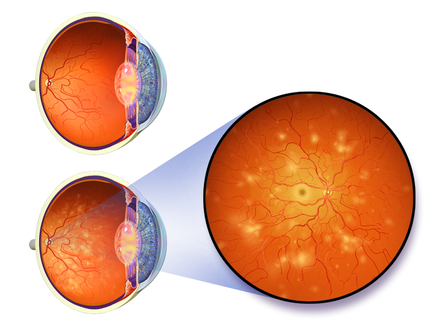
\includegraphics[scale=0.6]{images/illustration.png}
\caption{Diabetic retinopathy in comparison to a normal eye \cite{wiki}}
\label{eye}
\end{center}
\end{figure}

The primary cause of DR is that as a byproduct of the condition of diabetes, thinner blood vessels in the human body tend to form abnormal branching structures and thinning walls. This leads to either deteriorated blood supply to the effected areas or actual hemorrhaging. In terms of the retina, this leads to blind spots forming in the field of vision of the afflicted individual. 
To diagnose the condition, a retinal scan of the eye is taken and a classification is assigned depending on the number of abnormal vein branching, wall thickness of the blood vessels and blood stains observed. DR is categorized on a scale from 0 to 4, and examples of level 0 and 4 DR are given below. It should be noted that this method of categorizing DR is not fundamentally rigorous in nature and is more of a qualitative scale. 

\begin{figure}[htbp]
\begin{center}
 \subfigure[Level 0 DR]{\label{reference}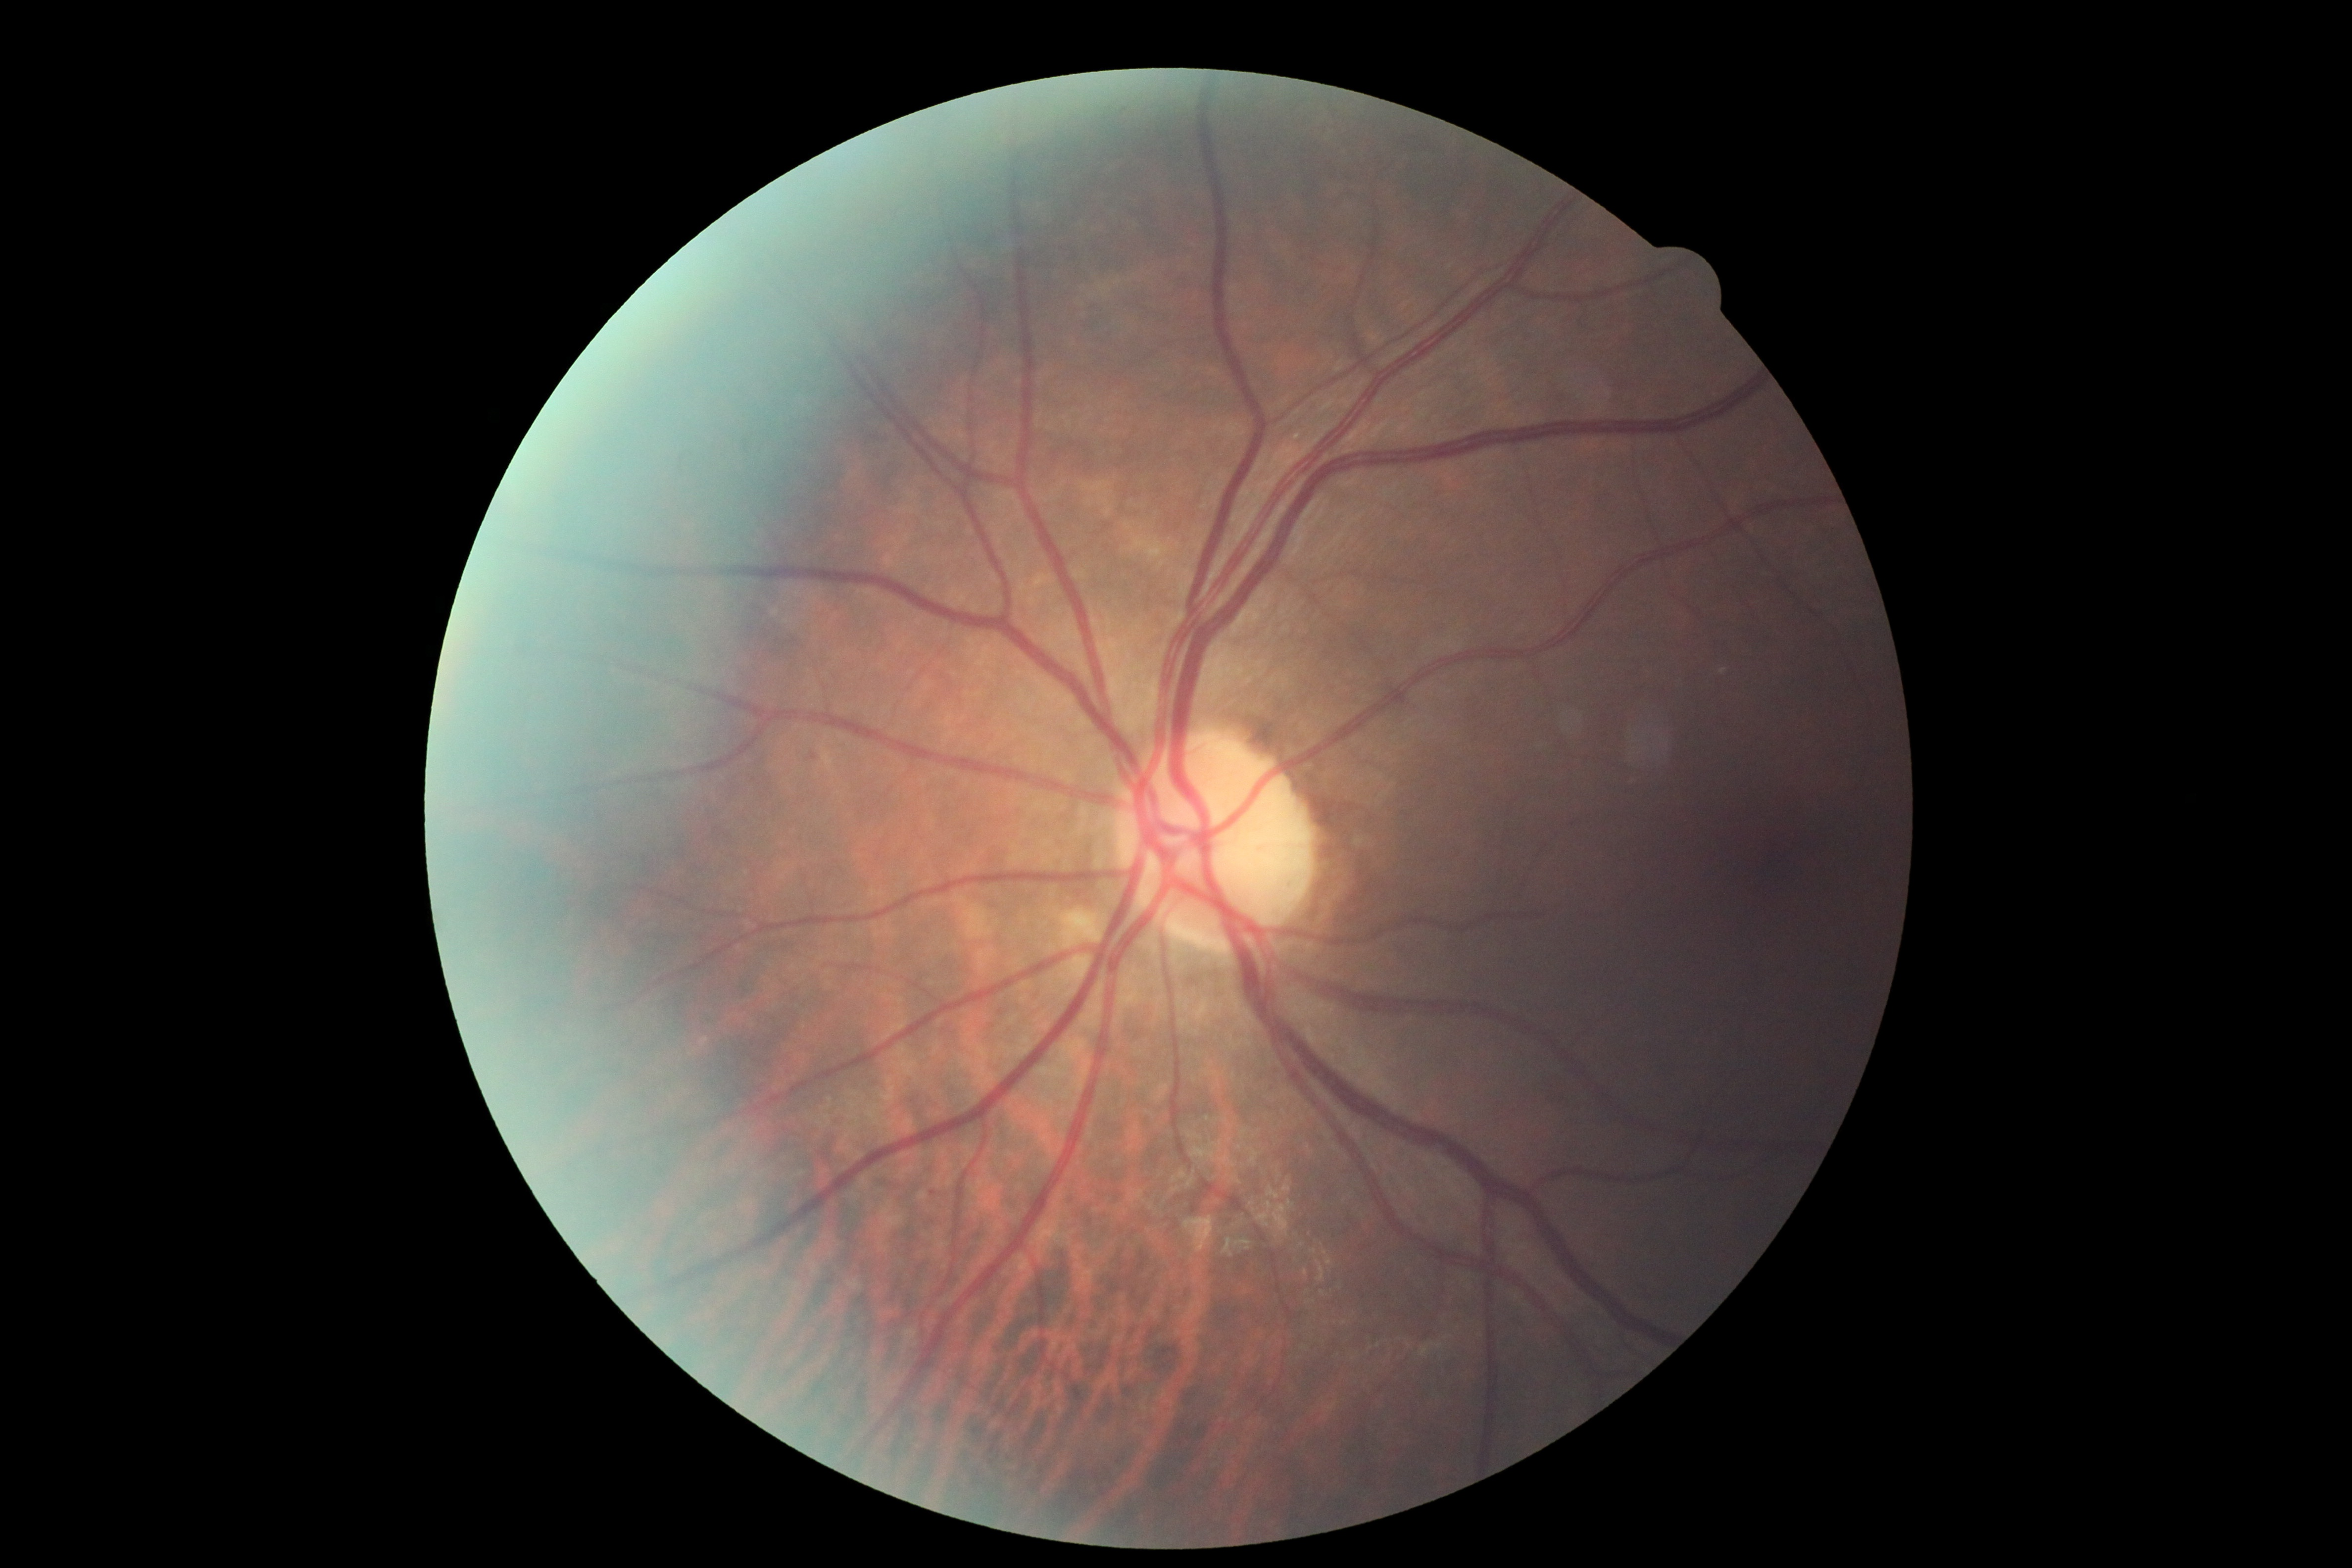
\includegraphics[scale=0.035]{images/0_Level_Example.jpeg}}
  \ \ \ \ 
\subfigure[Level 4 DR]{\label{new}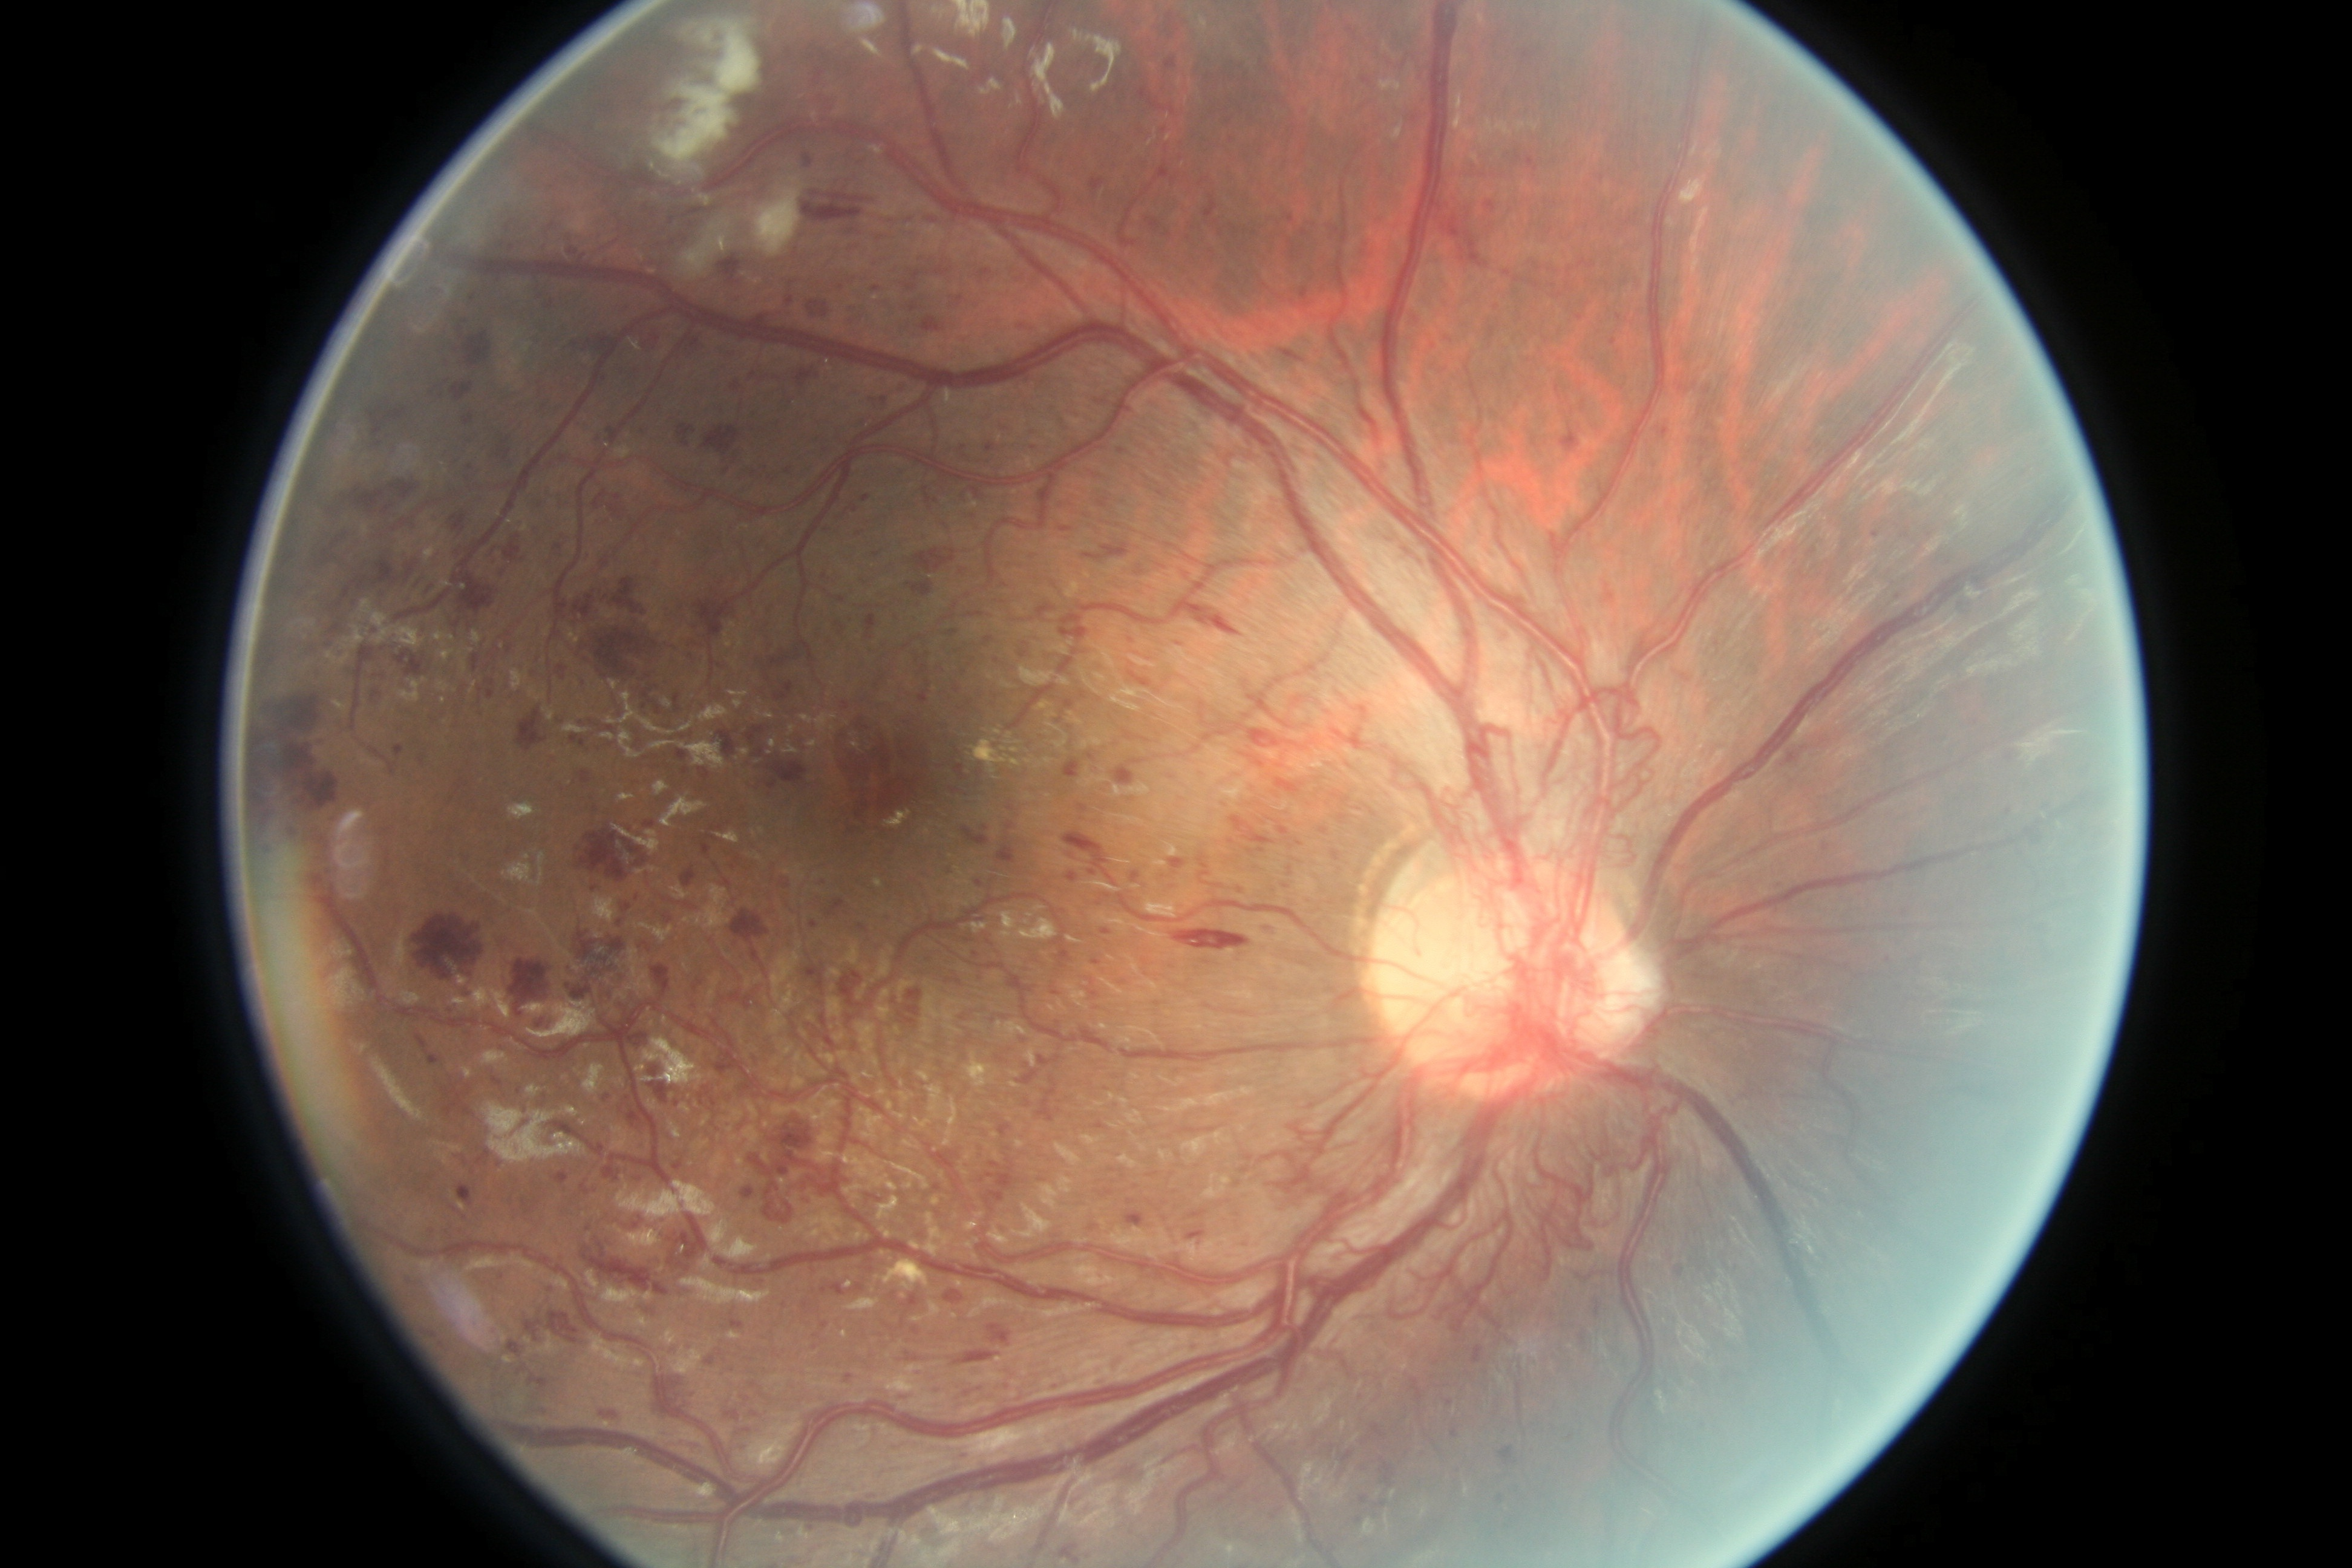
\includegraphics[scale=0.0425]{images/4_Level_Example.jpeg}}
\caption{Examples of level 0 and level 4 DR}
\label{marking_image}
\end{center}
\end{figure}

\subsection{The Kaggle Grand Challenge}

Kaggle has presented the automated DR diagnosis as open grand challenge. In doing so, Kaggle provided ~35 gigabytes of retinal scan data, over 35,000 images, thus each image is roughly 1.5 megabytes in size. To facilitate download and processing of the data set, Kaggle divided the image set into a training group, and a testing group, and the subsequently divided each group into smaller subsets to facilitate file transfer. All the results presented here and in subsequent discussions are based on the first training set of images.

It is noted that the aim of the current work is to understand ConvNN from a fundamental perspective, and not to actually create a competitive solution for the grand challenge. Due to the size of the reference data set, and the limitations imposed by Python in terms of loading elements into shared memory, it would be very difficult to create a code base that could compete directly with other implementations in CuDa, (a GPU-level system language), which is defacto favorite language for image processing.	

\section{Convolution Neural Networks}

ConvNN are a powerful machine learning technique that fall under the of general premise of deep learning. There are number of flavors of ConvNN, but the specific implementation presented here is one of the first implementations of the technique, the LeNet-5 \cite{LeNet}, and is especially adept at processing digital imaging.

The LeNet-5 consists of 3 primary component layers: the convolution layer, the pooling layer, the conventional fully connected layer \cite{deep}. 

\subsection{The Convolution Layer}

The convolution layer is the work horse of the ConvNN, and it is what makes it such an indispensable tool for image processing. Mathematically, the concept of convolution is somewhat straightforward, and plays a key role in spectral methods and Fourier space treatments. In terms of digital imaging, convolution can be expressed as \cite{deep} the product of the pixel intensity of a given image with that of a kernel, and is stated as
\begin{equation}
H[m,n] * G[m,n] \, = \, \sum_{u=- \infty}^{\infty} \sum_{u=- \infty}^{\infty} H[u,v] G[m-u, n-v]
\end{equation}

This may seem somewhat complex at first, but consider that an image is an array of pixels, each with an intensity that ranges from 0 up to a given bit depth, (e.g. 255 for 8-bit images), than we can see that an image can be translated as matrix, where each element is a given pixel's image intensity. The concept is illustrated in \figref{lena}.
\begin{figure}[htbp]
\begin{center}
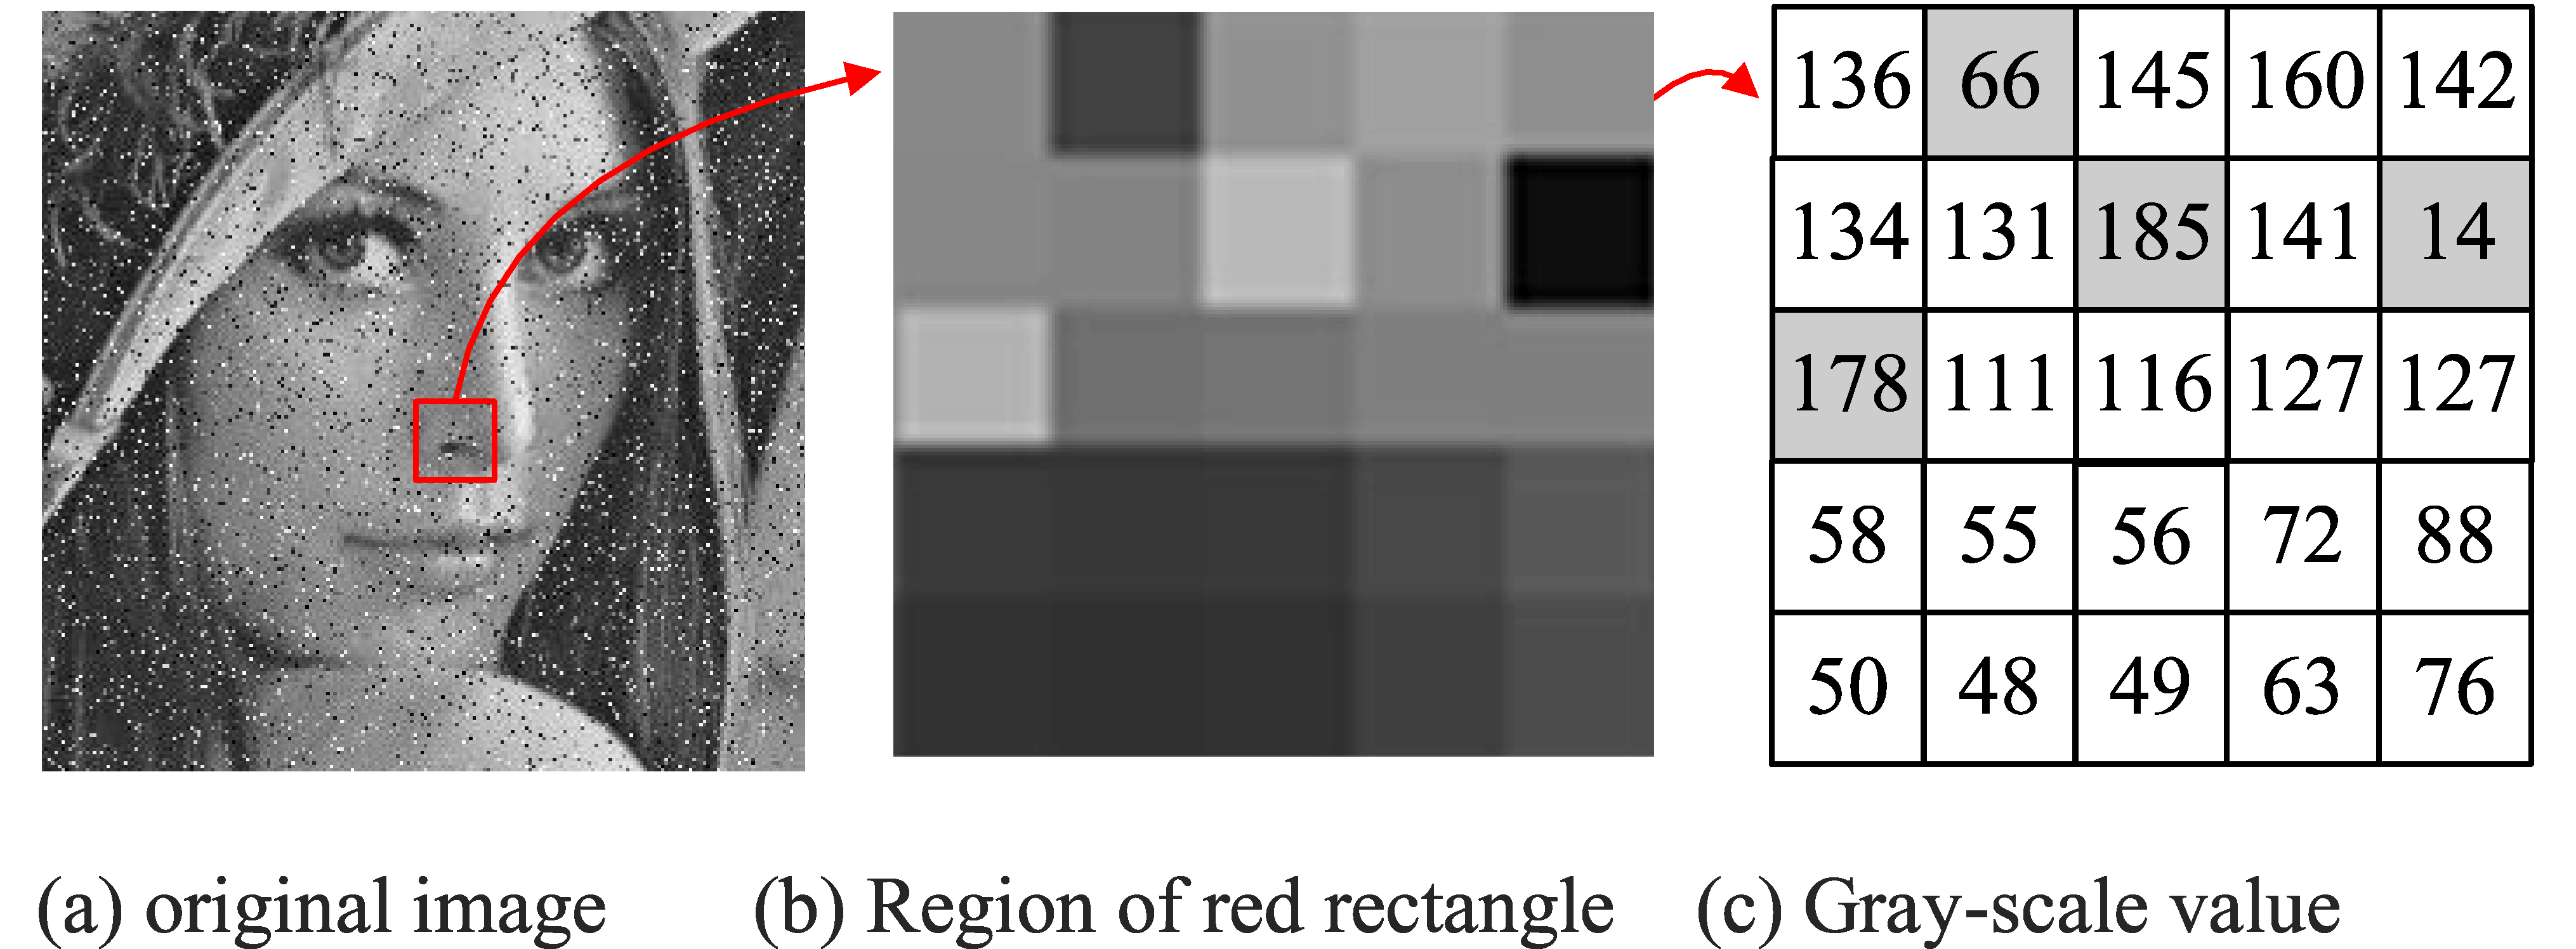
\includegraphics[scale=0.1]{images/lena.png}
\caption{Digital image as a matrix \cite{lena}}
\label{lena}
\end{center}
\end{figure}

With this concept in place, a kernel, is itself a matrix of a prescribed dimension, smaller than that of the original image,  an example of which would be
\begin{equation}
H_{3 \times 3}^L \, = 
\begin{bmatrix}
  0 & 1  & 0 \\
  1 & -4 & 1 \\
  0 & 1  & 0
\end{bmatrix}
\label{lap_3x3}
\end{equation}

This matrix is applied, via convolution, across the matrix of the image to create a filtered image which, depending on the \textit{stride}, (i.e. number of times the kernel is applied across the original image), downsizes the original image into smaller matrix which is representative of the dot product between the original image and kernel.  The full convolution concept is illustrated in \figref{conv}. At this point, the ConvNN is ready to pass this resulting matrix to a pooling layer

\begin{figure}[htbp]
\begin{center}
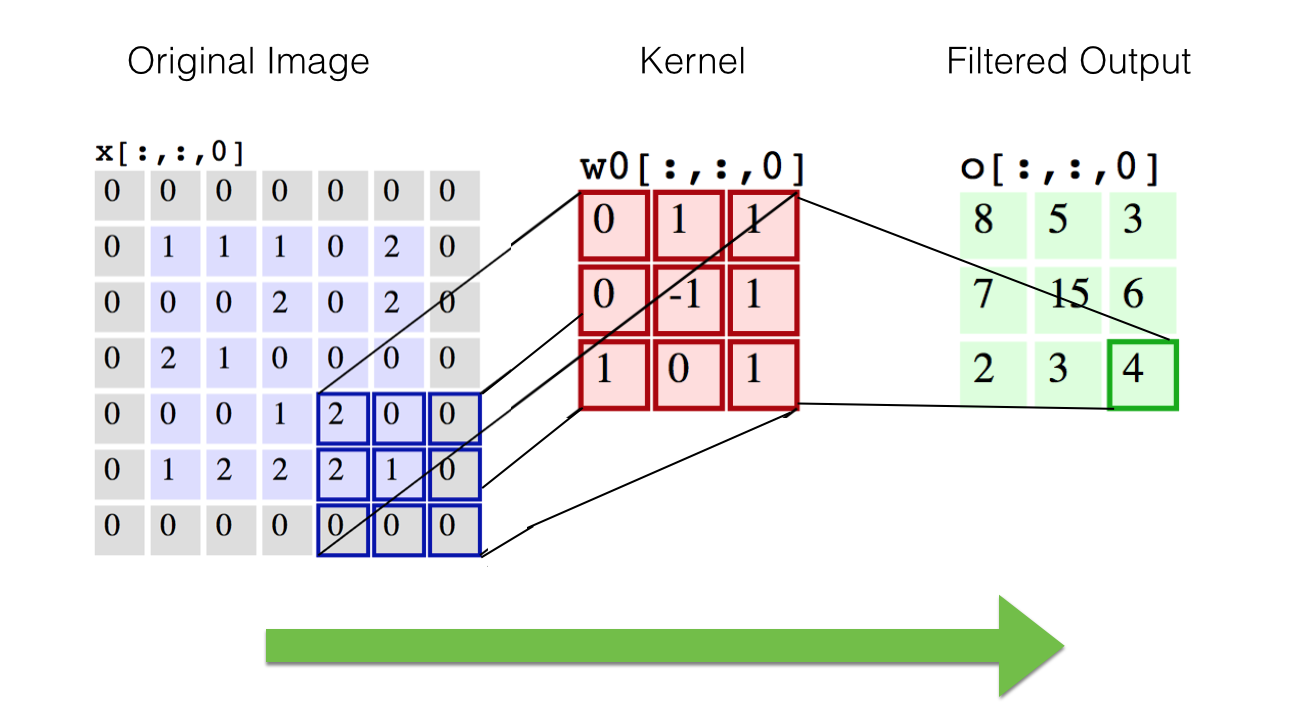
\includegraphics[scale=0.7]{images/convolution.png}
\caption{Convolution concept \cite{cs231}}
\label{conv}
\end{center}
\end{figure}

\subsection{The Pooling Layer}

In order to reduce the computational expenditure of the ConvNN algorithm, a pooling module is often used to reduce the required number of weights for a subsequent fully connected neural network layer.  

Usually the form of the pooling is \textit{max Pooling}, where  a specific number of elements of the convoluted image are defined as common-pool members, (as illustrated in \figref{maxPool}), and only the pool member with the maximum value is carried forward in the network. The size of a pool is usually, but not required to be, the same size as the kernel applied during convolution. By focusing on the maximum value of a convolution, the network is becoming more sensitive to those image features which are more dominant of the total feature set.

\begin{figure}[htbp]
\begin{center}
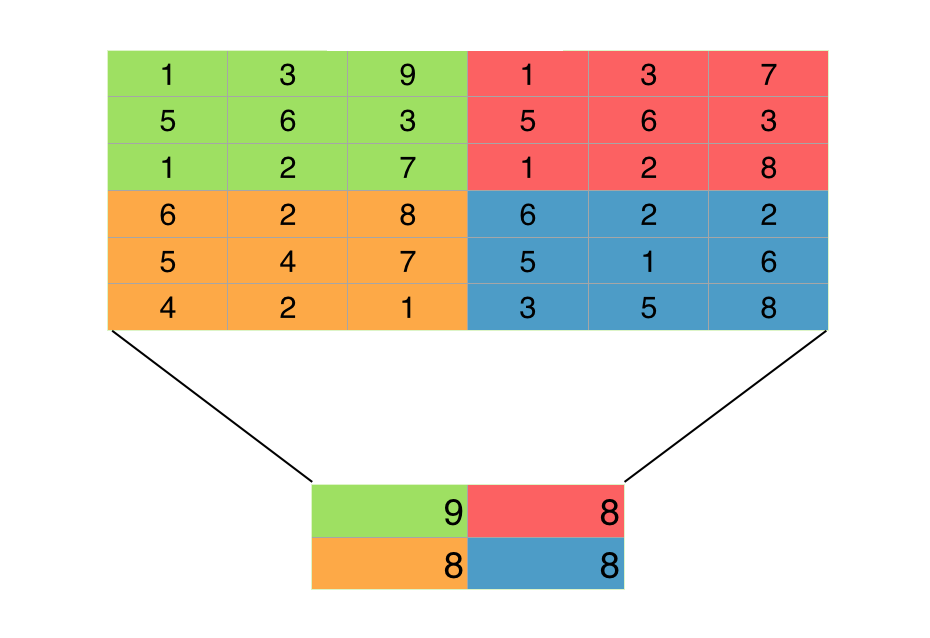
\includegraphics[scale=0.5]{images/maxpool.png}
\caption{Max-pooling: the largest value of each sub-cell is fed forward}
\label{conv}
\end{center}
\end{figure}

It is noted that a ConvNN often uses a series of convolution and pooling layers to continuously reduce the computational load of the final layer, or layers, of fully connected NN, which is normally the most computational expensive facet of the ConvNN pipeline. 

\subsection{The Fully Connected NN Layer}

The fully connected NN layer is actually what a \textit{conventional} neural network, which is comprised of a series of nodes that are interconnected via a series of weights and bias units. Let's begin with the illustration shown in \figref{ann}.

\begin{figure}[htbp]
\begin{center}
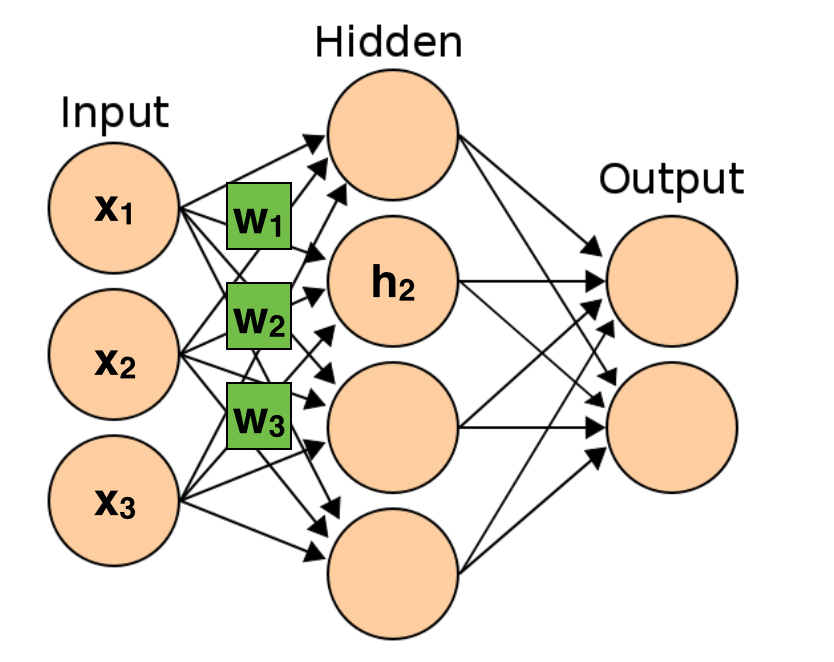
\includegraphics[scale=0.5]{images/nn_edit.png}
\caption{A fully connected neural network \cite{ann}}
\label{ann}
\end{center}
\end{figure}

As can bee seen from the figure, each node is connected to the series of nodes in the layer directly downstream of it. The node downstream is in turn connected to each node in the layer upstream of it, as well as each node in the layer downstream.

Let's say that for each input connection of a given node, there is an associated weight $w_i$. Given that there is $N$ number of nodes in the upstream layer, the input to node can be seen as 
\begin{equation}
f(\vec{w}^T\vec{x}) \, = f(w_0 \cdot x_0 + w_1 \cdot x_1 + \cdots + w_N \cdot x_N)
\end{equation}

We note that the dot product shown above is the input to a function, known as the activation function, that in turn is the input value of the downstream node. There are a variety of activation functions that can and have been used in NN. One of the most popular kind, and the one which is used here, is the \textit{tanh} activation function, which is defined as
\begin{equation}
f_{\text{tanh}}(a) \, = \frac{e^a-e^{-a}}{e^a+e^{-a}}
\end{equation}
which has an activation profile shown in \figref{} As can bee seen, the function has asymptotes  at 1 and -1 and exhibits positive values in $y$ for positive values of $x$. Another common activation function is the sigmoid activation function, which has a similar profile as \textit{tanh} and has the functional form
\begin{equation}
f_{sigmoid}(a) \, = \frac{1}{1-e^{-a}}
\end{equation}
The sigmoid activation function has asymptotes at 1 and 0, and is centered at the origin in $x$ and at 0.5 in $y$. 

These two functions are very similar in profile, but the \textit{tanh} function is more commonly used due to its favorable back-propagation properties, (i.e. the learning process of the NN). Back-propagation is a key concept to NN and ConvNN, but its description is beyond the scope of this first draft and will most likely be discussed in the final draft of the current document.

\subsection{Logistic Regression Node}

The final layer of the ConvNN is the logistic regression function node, which is a classifier we have reviewed in class. It's functional form is \cite{deep}
\begin{equation}
y_{prediction} \, = \, \text{argmax} P_i (Y = i | \{x, W\})
\end{equation}
where the probability is
\begin{equation}
P_i \, = \, \frac{e^{\vec{w}_i^T \vec{x}_i}}{\sum_j \vec{w}_j^T \vec{x}_j }
\end{equation}
This simply means that the output of the NN is mapped to one of the label of classes a given image may be categorized as, and the label which has the highest probability of matching of all the the potential outcomes becomes the label of the given option.

\section{Summary}

So putting all the pieces together of the ConvNN, we have the general layout seen in \figref{summary}

\begin{figure}[htbp]
\begin{center}
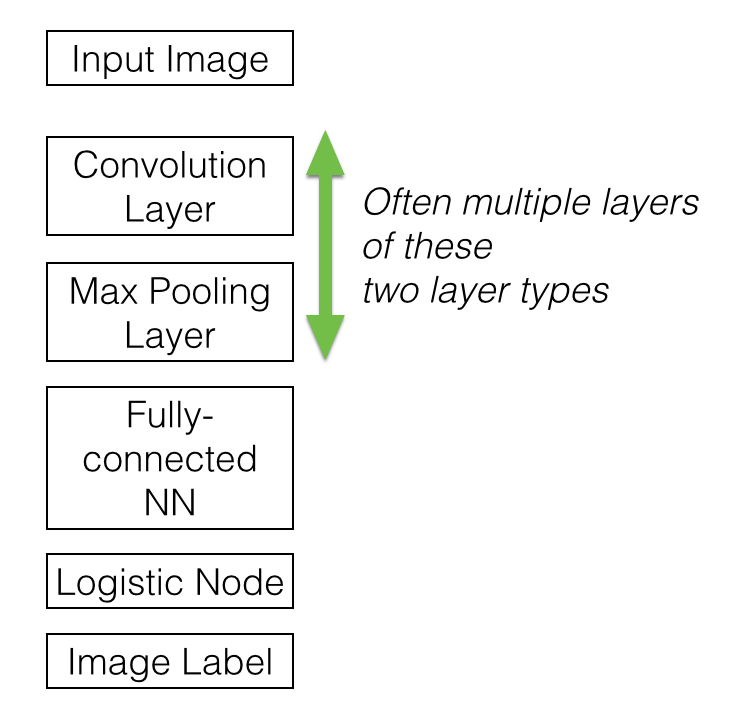
\includegraphics[scale=0.6]{images/summaryNN.png}
\caption{The ConvNN as a whole}
\label{summary}
\end{center}
\end{figure}

As noted in the figure, the convolution layer and the max pooling layer are often stacked multiple times in practice to reduce the overall computational load of the fully connected neural network module, which is often the most computational expensive member of the ConvNN. In the current work, two repetitive blocks of convolution layers and max pooling layers have been used to process the input image.

\section{Current Project Status}
\newpage
% \nocite{*}
\bibliographystyle{unsrt}
\bibliography{References}


\end{document}